\documentclass[12pt,a4paper]{article}

\usepackage{ctex}
\usepackage[paper=a4paper,includefoot,margin=54pt]{geometry}
\usepackage[colorlinks,linkcolor=black,anchorcolor=black,citecolor=black,unicode]{hyperref}
\usepackage{float}
\usepackage{listings}
\lstset{frame=single,breaklines=true,postbreak=\raisebox{0ex}[0ex][0ex]{\ensuremath{\hookrightarrow\space}}}

\renewcommand{\lstlistingname}{程序}
\renewcommand{\contentsname}{目录}
\renewcommand{\abstractname}{摘要}
\renewcommand{\refname}{参考文献}
\renewcommand{\indexname}{索引}
\renewcommand{\figurename}{图}
\renewcommand{\tablename}{表}
\renewcommand{\appendixname}{附录}

\begin{document}

\title{基于光栅的裸眼3D技术\\详细设计报告}
\author{王子博,赵子瑞,鲁吴越,李嘉豪}
\date{2017年6月}

\maketitle
\tableofcontents
\newpage

\section{架构设计}

我们最终提出的裸眼3D解决方案包含一块光栅屏、一个校准程序、一个视频播放程序和一套游戏画面渲染技术。用户应准备一个合适的显示设备,其上有固定的前置摄像头。将光栅屏覆盖于显示设备表面,并尽可能令光栅方向和屏幕像素排列方向平行后,用户可运行校准程序,完成其中的测试步骤。校准程序会测量出屏幕的一系列参数,将其存储于配置文件中。最后,用户可随时使用视频播放程序欣赏3D视频,或运行特定的游戏程序体验3D游戏。

对于3D视频,一般只能找到双图层的片源,为了改善观赏体验,前置摄像头可被用于实时追踪用户双眼位置,针对性地输出画面。如果禁用此功能,用户亦可在保持头部不动的前提下进行观赏。

对于3D游戏,视游戏引擎能力可产生双图层或多图层输出,其中以多图层为佳,此时无需使用双眼追踪功能即可自由体验,甚至在晃动头部时3D视觉感反而会增强。考虑到紧张刺激的游戏需要显示系统快速响应,以及用户时常会情不自禁地移动头部,避免启用双眼追踪可以大幅改善用户体验。若游戏引擎只能输出双图层图像,则应尽量启用双眼追踪功能,根据双眼位置调整游戏中摄像头位置,给用户更好的立体感。

\section{技术路线}

\subsection{3D视觉}

人的立体感主要有两种来源,一是\emph{双眼位置不同,所看到的画面有细微差异},经大脑叠加处理后所形成的立体感,我们称之为\emph{静立体感},如图\ref{static3d}%
\begin{figure}[htbp]
\begin{minipage}[t]{0.5\linewidth}
    \centering
    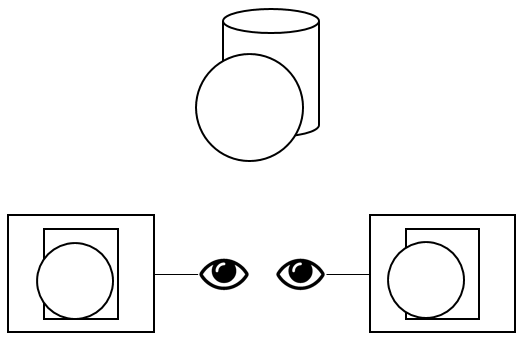
\includegraphics[width=0.8\linewidth]{2}
    \caption{静立体感的形成}
    \label{static3d}
\end{minipage}
\begin{minipage}[t]{0.5\linewidth}
    \centering
    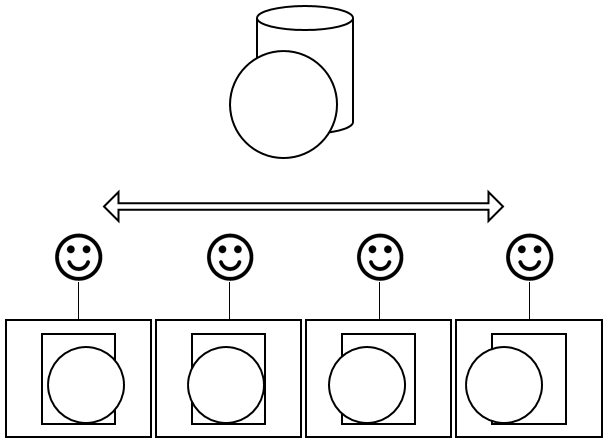
\includegraphics[width=0.8\linewidth]{3}
    \caption{动立体感的形成}
    \label{dynamic3d}
\end{minipage}
\end{figure}%
;二是\emph{移动头部时由于视点变化,所看到的画面逐渐改变}所带来的立体感,我们称之为\emph{动立体感},如图\ref{dynamic3d}。

静立体感需要为双眼各提供一份图案,我们称之为\emph{图层},一个图层就是从一个视点拍摄出的一列随时间变化的图像。而动立体感有两种解决方案,一是准备若干个图层(一般为十个到几十个),对应于不同视点所拍摄出的图像,视每只眼睛当前所在的位置决定其具体看到的图层;二是动态追踪眼球所在位置,实时计算出在该位置时应当看到的内容。后一种方案只需要渲染两个图层(它们的视点都在随用户眼球位置变化),但需要实时完成人脸识别、眼球定位和分析,将GPU开销转化为了CPU开销。

\subsection{光栅分光}

要从一块屏幕向两只眼睛分别显示出不同的内容,必须有某种分光手段,使得射出的光线沿特定方向传播,仅被处于特定区域的眼睛所看到。这种分光手段就是我们项目的核心——光栅。为了研究光栅的光学特性,我们自行开发了名为GASP (Grating Advanced Simulation Platform)的平台。该平台分析的结论概要如下:

图\ref{4}%
\begin{figure}[htbp]
\begin{minipage}[t]{0.5\linewidth}
    \centering
    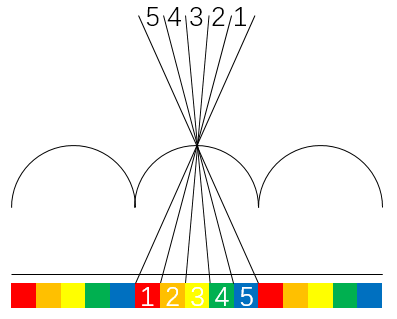
\includegraphics[width=0.8\linewidth]{4}
    \caption{理想光栅,PPL=5}
    \label{4}
\end{minipage}
\begin{minipage}[t]{0.5\linewidth}
    \centering
    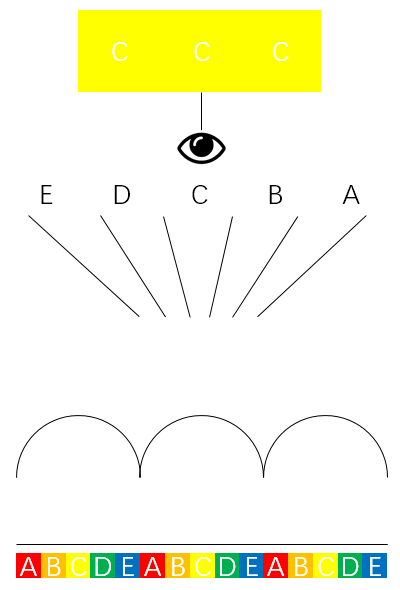
\includegraphics[width=0.8\linewidth]{5}
    \caption{PPL=5的光栅效果}
    \label{5}
\end{minipage}
\end{figure}%
展示了一个理想情形下的光栅,它可以被视为一系列柱形透镜,能将其下的像素投射到空间中特定位置。图中的光栅每条透镜覆盖了5列像素,我们称5为这个屏幕的PPL值,因此在空间中形成了5种区域,眼睛处在任何一个区域内时,都只能看到相应的1列像素的颜色。

若在第0、5、10、15……列像素显示图像A,第1、6、11、16……列像素显示图像B,以此类推,则在整个显示屏外的空间中产生若干个区域,如图\ref{5}。任何一个区域内的眼睛只能看到相应的一幅图像。这就实现了分光。

然而,现实中的光栅应用场景不够理想,这主要是因为现有的显示屏表面总是覆盖了一定厚度的保护层,导致光栅底部不能完全贴合显示表面,对焦出现偏差。重新开模制作更薄一些的光栅板可以彻底解决这个问题。目前我们模拟得知,在这种对焦出现偏差的情形下,光栅无法做到只投射出1列像素,而是会投射出多列像素。如果为3列,我们称3为这个屏幕的WPL值,则每条光栅上总会左右颠倒地显示出3列像素,用户在不同位置看到的图案分别如图\ref{6}%
\begin{figure}[htbp]
    \centering
    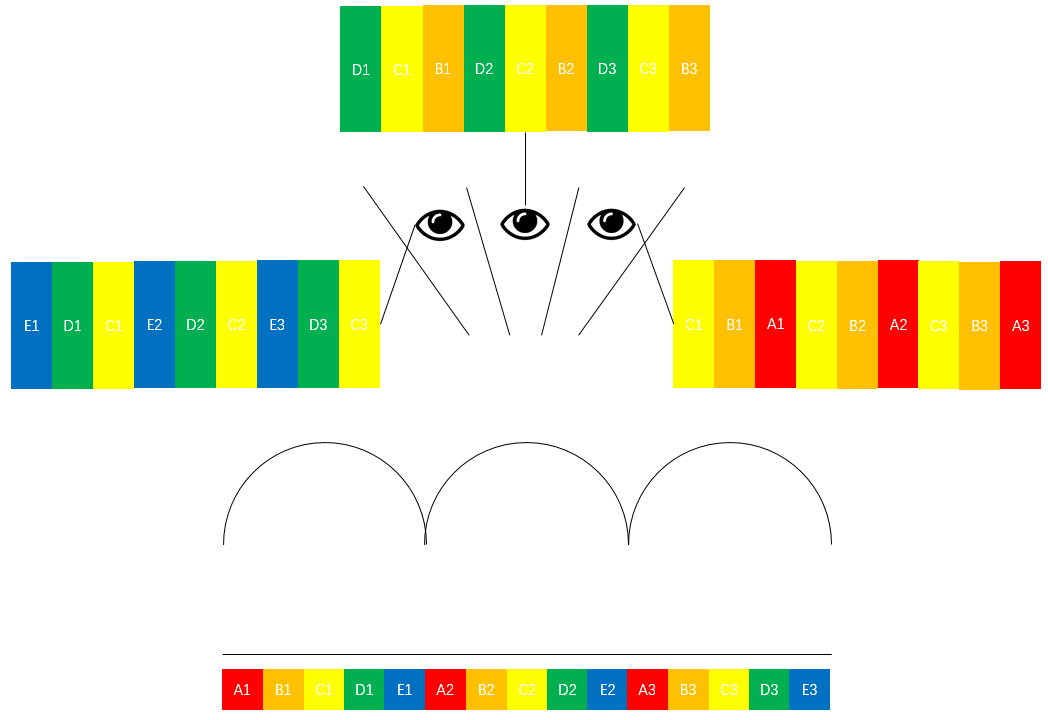
\includegraphics[width=\linewidth]{6}
    \caption{PPL=5,WPL=3的光栅效果}
    \label{6}
\end{figure}%
。

\subsection{双图层与多图层}

在理想情况下,光栅可以在空间制造出若干个扇形区域,每个区域内的眼睛只会看到特定的一些像素(它们的列数模PPL同余)所拼成的图像。此时,若能从PPL个不同的视点拍摄物体,将所得图像放在相应的像素上显示,即可产生一副PPL张图像的混合图像,我们称这种情形为多图层显示。由于观察者的双眼落在不同扇形区域内,双眼看到的不是同一张图像,因此会产生静立体感。而当观察者移动位置时,会看到和刚才不同的新图像,这会产生动立体感。这是最理想的一种情形,3D立体画即是用这种手段制作而成的,其PPL一般为10--20。

需要说明的是,空间中实际上会产生许多扇形区域,其中每相邻的PPL个扇形区域为一个循环,如图\ref{7}%
\begin{figure}[htbp]
    \centering
    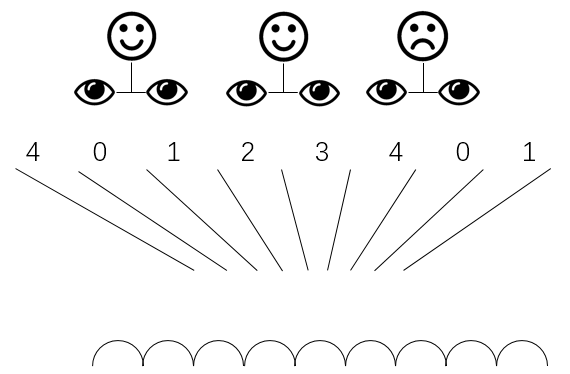
\includegraphics[width=0.6\linewidth]{7}
    \caption{PPL=5,WPL=1,DOE=1的情形}
    \label{7}
\end{figure}%
。观察者的左右眼所处的区域编号一般有一个常数差值,如1,我们称这个1为DOE。则当其左眼看到0号图层时,右眼正在看1号图层;当其左眼看到1号图层时,右眼正在看2号图层……当其左眼看到4号图层时,右眼正在看0号图层---这时显示效果是错误的!一般来说,会产生这种错误效果的区域占所有区域的比例为DOE/PPL。当PPL很大时,这个问题并不明显,无需在意。但当PPL为2时问题就会变得很严重,以至于观察者绝对不可以移动头部,否则将会看到错误的显示效果。因为一般能找到的3D电影片源都只有两个图层,而PPL为2时存在这种特殊性质,我们将双图层情形独立出来专门研究。

如果只有两个图层,而观察者又有可能移动视角,我们就需要实时检测观察者当前眼睛所在的位置,并据此动态调整显示方案以“追上”观察者。

\subsection{实时双眼追踪}

双图层时实时双眼追踪来更正显示的原理如图\ref{8}%
\begin{figure}[htbp]
    \centering
    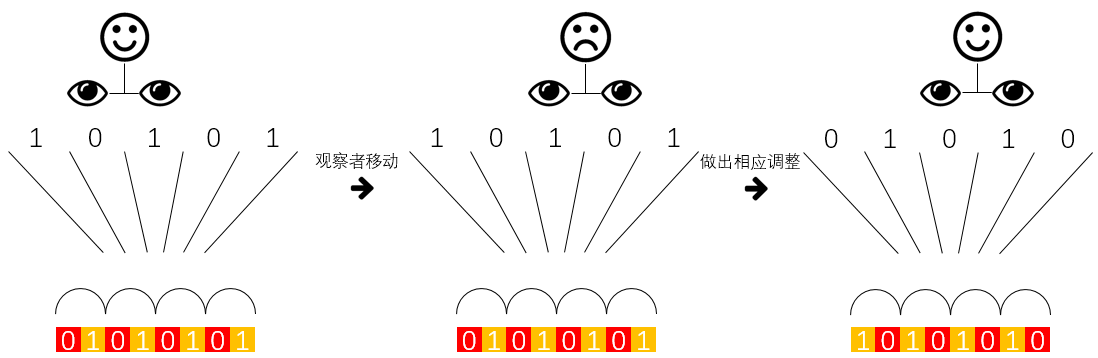
\includegraphics[width=\linewidth]{8}
    \caption{在观察者移动头部后,系统根据人眼追踪的结果重新安排了图层顺序}
    \label{8}
\end{figure}%
。我们在OpenCV的人脸识别库基础上自行开发了名为GOD (Grating OpenCV-based Detector)的人眼定位与追踪系统,它能在面孔上合适范围内寻找黑色虹膜区域(对其他眼睛颜色的用户或黑色皮肤用户可能无效),并按照人的一般运动规律预测性地寻找接下来眼睛的移动轨迹。

人眼追踪系统得出的人眼位置横坐标与该眼睛当前看到的图层编号间近似为简单线性关系。在校对程序中,用户需要标记可恰好看到0号图层的两个不同位置,程序即可自动求解出线性方程参数Period和Offset,并以此控制显示。

\subsection{校准}

一个特定屏幕的特性需要由4个参量刻画:PPL、WPL、Period和Offset。校准程序通过3步简单的测试实现了对这些参量的测量。由于在校准刚开始时我们对这些参量一无所知,此时很难在覆盖了光栅板的屏幕上显示文字供用户阅读,我们自行开发了名为SVIP (Grating Science Staged Visualized Integrated Platform)的平台进行校准。这个平台能清晰地显示出指引文本和测试图案,并能轻松地添加或修改测试步骤。

\subsection{显示}

为了最终进行图像渲染输出,我们自行开发了名为OGRF (OpenGL-based Grating Render Framework)的渲染引擎。它能根据测出的屏幕参量和实时人眼追踪的结果渲染画面。

\section{创新点分析}

这个项目的核心创新点在于借助一系列我们开发的软件,用户可以以低廉的价格购买光栅板,置于自己已有的任何显示屏前享受裸眼3D体验。为了尽可能改善使用体验,我们独创了多种技术手段,例如当光栅略有失焦,导致WPL不为1时,我们研究了光栅的显示特性,使软件输出反而更高分辨率的良好图像。当用户想播放只有双图层的片源时,借助于实时双眼追踪技术,我们的程序在提高输出精度的同时,对用户移动头部的适应能力增强,使用户舒适观影。相比之下,目前市面上其他类似产品价格昂贵、只能播放特殊影片或运行特殊游戏、对观察视角限制严格,不利于裸眼3D普及。

\section{各模块设计}

\subsection{测试环境}

目前尚未实现项目向安卓平台的移植,因此测试环境由一台手机、一个有前置摄像头的笔记本电脑、一块光栅板构成。笔记本电脑负责进行人眼追踪和渲染输出,其上运行了VNC服务器程序。手机和笔记本电脑接入同一无线网络,通过VNC客户端程序获得笔记本电脑的屏幕图像,以1:1显示。光栅板、手机、笔记本电脑三者一旦安装好就不可移动,否则人眼追踪需要重新校准。

在此测试环境下,我们已经尝试分别启用和禁用人眼追踪功能播放了双图层片源、多图层片源和运行了游戏。人眼追踪运行效果良好,唯一不足就是网络传送画面略有延迟,降低了人眼追踪的响应性,但这可通过将程序移植到安卓平台上解决。

\subsection{GASP}

Grating Advanced Simulation Platform是用Python和pygame库编写的一套光学模拟平台,可模拟各种光学成像现象,被用于研究光栅的光学性质。它含有一个无限大的工作区,用户可在其中摆放若干个物点(可用不同颜色分组进行区分)、光学器件(透镜、平面镜、光栅等),它会实时计算出所有可能的光路和产生的像点位置。

\begin{figure}[H]
    \centering
    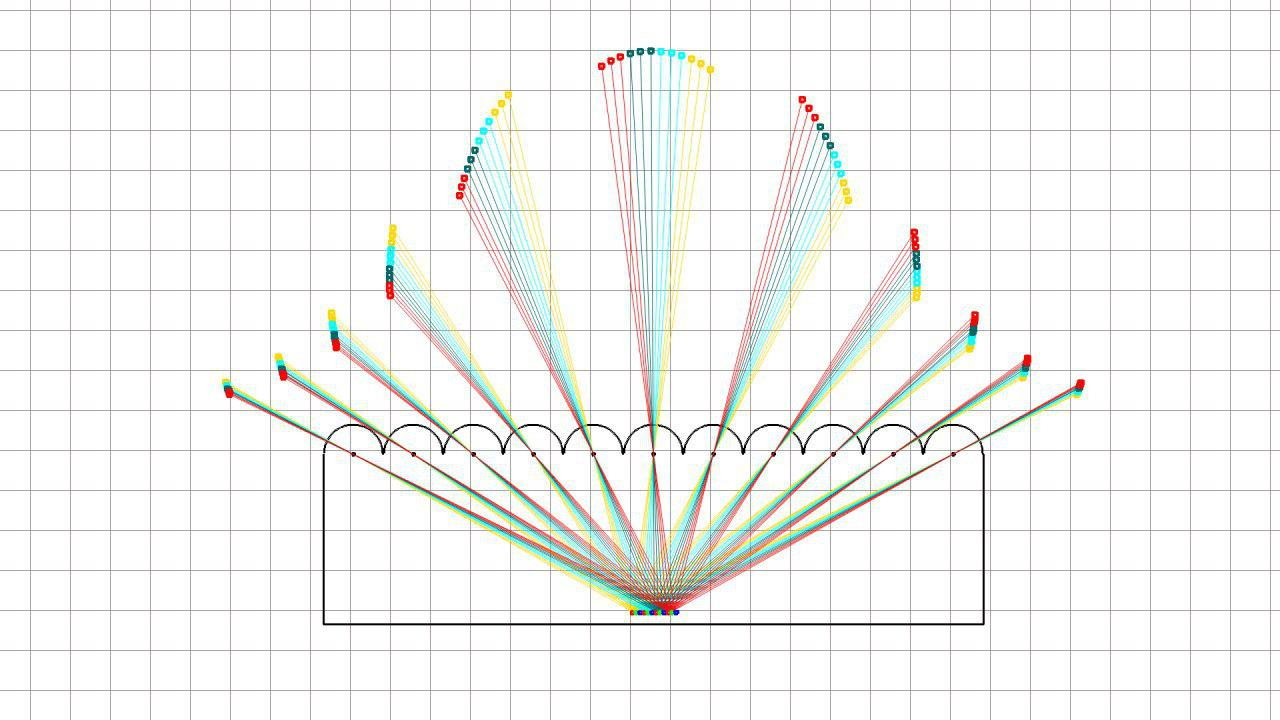
\includegraphics[width=0.8\linewidth]{gasp}
    \caption{GASP截图}
\end{figure}



\subsection{GOD}

Grating OpenCV-based Detector是用Python和OpenCV库编写的一套人眼追踪系统,可读取摄像头捕捉到的画面并追踪其中的人眼,被用于校准程序和改进视频播放和游戏渲染质量。它每个时刻都在上一时刻的眼睛位置附近寻找一个平均色调最暗的矩形区域,作为新的眼睛位置。由于人移动时加速度不会超过一定值,它会分析一小段时间内眼睛移动的速度矢量,来匀速预测下一时刻的眼睛位置,以此提高追踪精度。在程序刚启动时,以及检测到追踪失败时,它需要有额外手段来重新定位人眼,目前我们设计了两种手段:一是调用OpenCV自带的人脸识别库找出人脸位置,在此结果基础上定位到双眼,二是显示出摄像头捕捉的画面,由用户用鼠标手工指出眼睛位置。前者用户体验较好,但可靠性不如后者,因此在校准程序中我们使用了后者,而在播放视频、运行游戏时使用前者。

\begin{figure}[H]
    \centering
    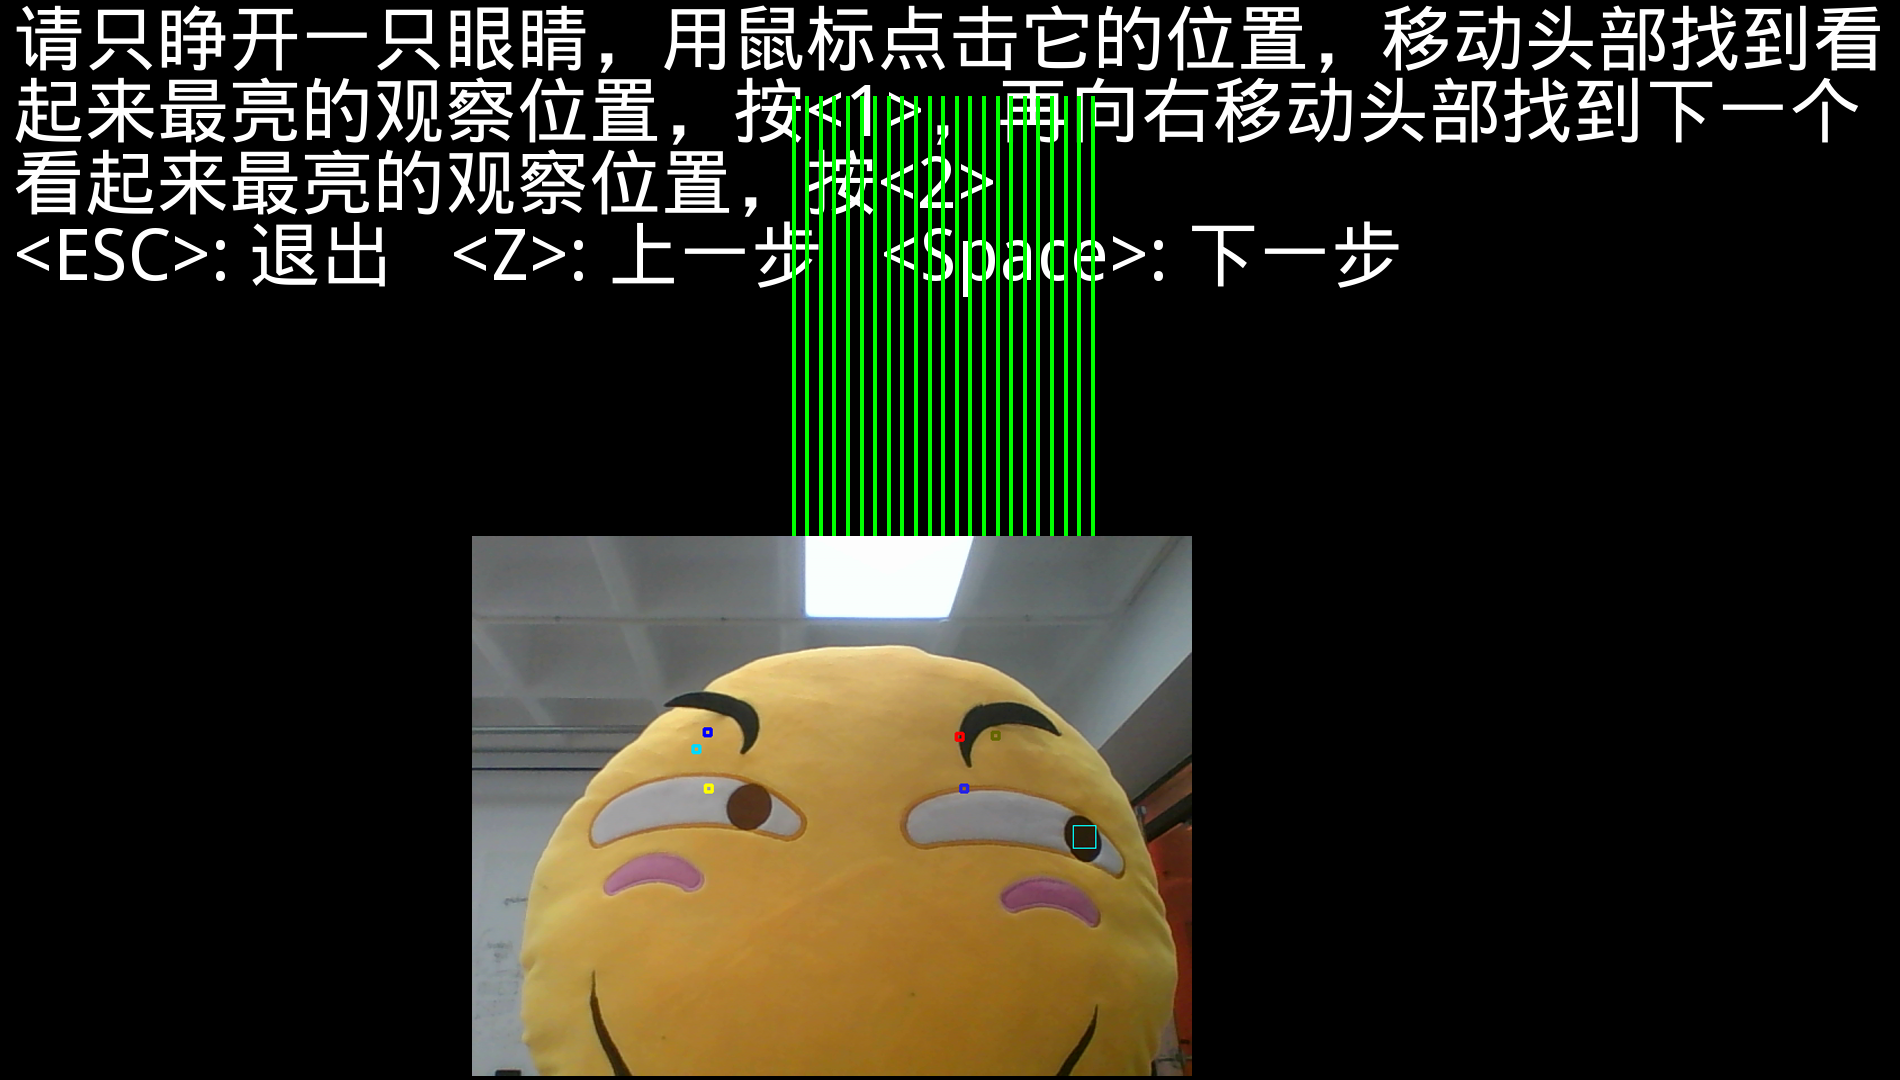
\includegraphics[width=0.8\linewidth]{god}
    \caption{在SVIP中出现的GOD界面}
\end{figure}



\subsection{SVIP}

Grating Science Staged Visualized Integrated Platform是用Python和pygame库编写的一套校准框架,可按步骤执行一系列校准任务并保存最终结果,被用于测量新屏幕的参数和初始化人眼追踪系统。尚未对屏幕进行校准时,一般应用程序很难显示文字供用户阅读,需要使用“抖动”的手法来提高文字清晰度。这个平台可以使编写校准任务简化,只需提供文字内容、校准图案和按键绑定,即可自动抖动文字、按顺序连接各步骤、收集测量结果并保存到文件。目前校准需要三步:第一步,通过莫尔条纹干涉法测量出PPL;第二步,通过观察找出WPL值;第三步,摄像头启动,用户找到能恰好看到0号图层的两个位置后,手工标记出相应的眼睛位置,系统算出Period和Offset。

\subsection{OGRF}

OpenGL-based Grating Render Framework是用C++和OpenGL库编写的一套渲染引擎,可给定屏幕参数和人眼追踪结果,产生出显示图案,被用于测试游戏的运行效果。它的核心变量是一个叫MASK的、长度为floor(PPL)的序列,其中记录了每一列像素从属的图层编号。如当PPL=11.4、WPL=3时,若人眼追踪结果表明当前左眼能看到4、5、6列像素,右眼能看到0、1、2列像素,则MASK=22201110000。显示时,所有floor(11.4n)列像素都是“循环节”的起点(也就是0、11、22、34、45……列像素),每个循环节宽11像素,其中各像素所从属的图层由MASK决定。注意有一些像素列,如33列,不属于任何一个循环节。

\begin{figure}[H]
    \centering
    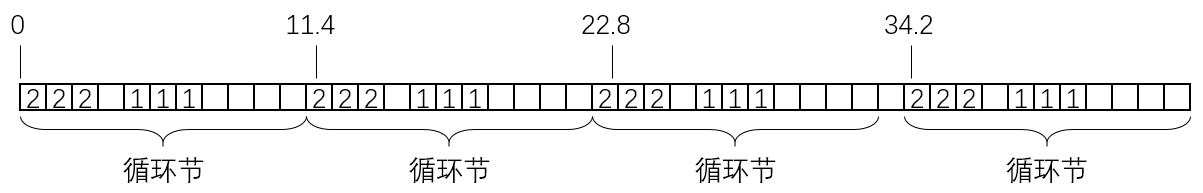
\includegraphics[width=0.8\linewidth]{ogrf}
    \caption{文本中所描述情形的渲染方式}
\end{figure}



\section{系统性能分析}

\subsection{效率}

无论是播放视频还是运行游戏,效率都是非常重要的。播放视频的要求较低,一般来说达到20余FPS即可,但运行游戏的要求较高,一般至少应达到60FPS。经过测试,目前由Python编写的、启用了人眼追踪的测试游戏程序,在中等配置的笔记本电脑上亦可满足此要求(至少70FPS),考虑到可用C++编写人眼追踪系统中的核心函数,效率一般能提高近十倍,本系统在笔记本电脑和台式机上的运行效率不会有问题。不过,在手机上的效率可能较低---在手机上运行本系统有两种方案,一是以笔记本电脑或台式机作为主机,完成运算并将图像传送到手机屏幕;二是直接在手机上完成运算并显示画面。前者受到网络延迟影响,后者受到手机计算能力影响。因此,在手机上运行,应当考虑禁用人眼追踪功能。

\subsection{稳定性}

我们实现的人眼追踪功能具有相当好的稳定性与响应性,经过测试,当观察者移动头部时,人眼追踪系统几乎总能立刻作出响应,正确预计移动轨迹。而当追踪失去目标时,内置的检验系统会在10帧内发现错误并重新开始定位,整个过程无需用户干预,最大化保证了用户体验的顺畅。

\subsection{可访问性}

这套解决方案的最大优势即是其可访问性---一块光栅板能用于一大批参数相似的显示屏,而且校准只需不到一分钟,用户可以随用随贴,随时揭下,灵活方便,免去了专门购买特殊设备的花费,也方便了游戏开发者为各种不同设备开发兼容游戏。


\end{document}
